\documentclass[letterpaper,10pt]{article}

\usepackage[english]{babel}
\usepackage[utf8]{inputenc}
\usepackage{amsmath}
\usepackage{graphicx}
\usepackage[colorinlistoftodos]{todonotes}
\usepackage[top=1in, bottom=0.9in, left=1in, right=1in]{geometry}
\usepackage[small]{titlesec}

\newcommand{\bes}{\begin{equation*}}
\newcommand{\ben}[1]{\begin{equation}\label{#1}}
\newcommand{\ees}{\end{equation*}}
\newcommand{\be}{\begin{equation}}
\newcommand{\ee}{\end{equation}}

\begin{document}

\begin{flushright}
{\Large Josh Bevan - HW 5 Q2 - CS556}
\end{flushright}
\vskip -0.1in
\hrule
\vskip 0.3in

\section*{Does convergence improve or deteriorate as the number of smoothing sweeps increases?}
Figure 1 plots the instantaneous convergence factors for a problem of size $2^{10}-1$ (with $kmax=10$ and $kmin=2$) with 1 to 10 smoothing passes of weighted Jacobi and Gauss-Seidel at a particular iteration. Generally as the number of smoothing passes increases the convergence factor is superior. There is a small variance in this behavior for Gauss-Seidel, but this is likely to do with fluctuations in the instantaneous convergence factor. The largest benefits are realized for increasing the number of passes from 1 to 2 for both smoothing methods. 

Using a Gauss-Seidel smoother yields a far superior convergence rate pass-for-pass compared to weighted Jacobi. In fact 6 passes of weighted Jacobi yields the same convergence rate as only 1 pass of Gauss-Seidel. This shouldn't be surprising considering Gauss-Seidel uses information from the full lower triangular part of $\mathbf{A}$, versus just the diagonal for weighted Jacobi. In general the spectral radius of the iteration matrix for Gauss-Seidel is smaller than for Jacobi when the methods are convergent. Indeed for the special case of a tridiagonal problem Gauss-Seidel converges at twice the rate as Jacobi. \footnote{A. Ralston and P. Rabinowitz, A First Course in Numerical Analysis, 2nd edition, McGraw-Hill, New York, 1978.} \footnote{D. M. Young, Iterative Solution of Large Linear Systems, Academic Press, New York, 1971.} Though we don't have this special case here, it does qualitatively point to the superiority of Gauss-Seidel. The question remains, however, if it is worth the cost.

\begin{figure}[!htb]
\centering
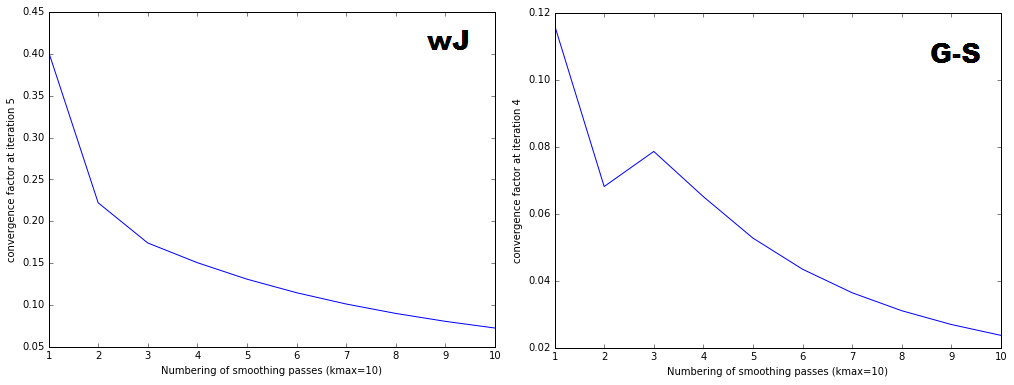
\includegraphics[width=1\textwidth]{cnvgJG.PNG}
\caption{Convergence factor at a particular iteration for various numbers of smoothing passes.}
\end{figure}

\section*{ Is it worth the cost? Compare weighted Jacobi versus Gauss-Seidel.}
Similar to the approach taken in Question 1, the time evolution of the residual is plotted for both smoothers in Figure 2 to examine their efficiency. Figure 3 presents the final residual after all iterations. Figure 3 is an easier to view plot than Figure 2 for the purposes of determining efficiency, but the elapsed time to reach the final iteration is not the same for all runs (as a fraction of an iteration does not make sense); care must be taken to examine Figure 2 to ensure that a given run does not reach a lower final residual merely because the final iteration greatly exceeded the nominal runtime. For the cases and problem studied it is clear from Figure 2 that this is not a concern for the most efficient configuration for each smoother, so we will now more closely examine Figure 3.

For weighted Jacobi the most efficient number of smoothing passes was 2, achieving an order of magnitude lower residual in the same time as using just 1 pass. Any more passes and the cost can not be justified for the meager increase in convergence factor. In contrast 1 pass of Gauss-Seidel was the most time efficient number. Despite 2 passes of Gauss-Seidel having almost double the convergence factor it still wasn't more efficient, most likely because (unlike weighted Jacobi) the cost of the smoother is now a more appreciable fraction of the overall cost compared to the v-cycle.

We can now compare the most efficient number of passes for both smoothers to determine the better smoother for the problem studied. Two pass weighted Jacobi yielded a residual of 2.33e-06 after 30 seconds of runtime compared to a residual of 6.21e-10 for single pass Gauss-Seidel. Therefore the extra cost of Gauss-Seidel is more than balanced out by it's superior convergence factor, making it the more efficient choice for this problem.

One important implementation note is that the smoothers were implemented via a scipy.sparse.linalg.spsolve(). Notably weighted Jacobi can be implemented with a lower overhead since the diagonal is trivially invertible, however when this method was used the convergence factor of the overall multigrid solver decreased as the V-cycle depth increased, much beyond what was attributed to the direct solving of a smaller but more approximate system at a coarser level. The likely cause of this is some form of numerical sensitivity that was avoided in the spsolve() version. This in principle could effect the efficiency of weighted Jacobi compared to Gauss-Seidel, but the difference in execution speed amounted to approximately 20\% in practice which left the relative ranking of performance unchanged.

\begin{figure}[!htb]
\centering
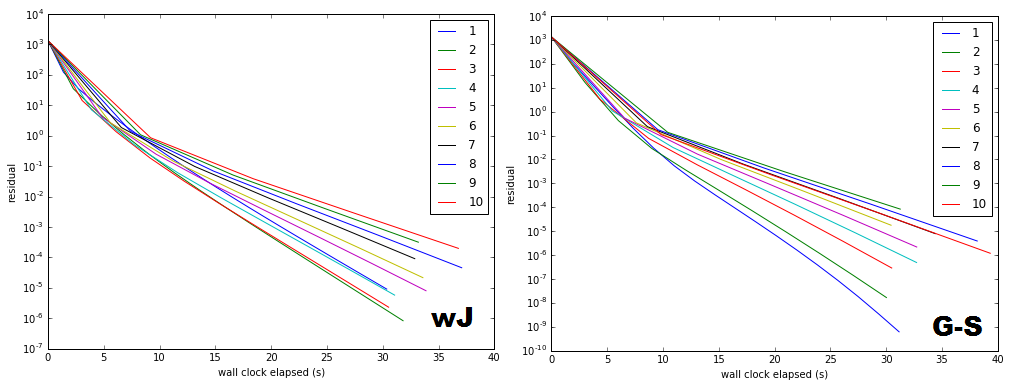
\includegraphics[width=1\textwidth]{restimeJG.PNG}
\caption{Wall clock time evolution of log of residual for various numbers of smoothing passes.}
\end{figure}

\begin{figure}[!htb]
\centering
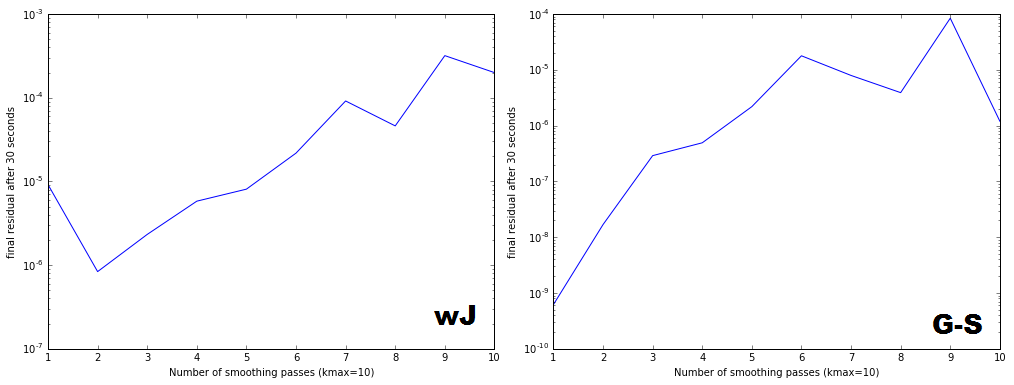
\includegraphics[width=1\textwidth]{resfJG.PNG}
\caption{Log plot of residual for various numbers of smoothing passes, all of which have been allowed to run for 30 seconds.}
\end{figure}

\end{document}
